\documentclass[12pt,a4paper,onecolumn]{article}
\usepackage{amsfonts}
\usepackage{graphicx}
\usepackage{listings}
\usepackage{array}
\usepackage{enumitem}
\usepackage[svgnames]{xcolor}

\addtolength{\oddsidemargin}{-0.5cm}
\addtolength{\evensidemargin}{-0.5cm}
\addtolength{\textwidth}{1.0cm}

\addtolength{\topmargin}{-1.5cm}
\addtolength{\textheight}{2.5cm}

\begin{document}

\lstset{ %
  backgroundcolor=\color[rgb]{0.95,0.95,1.0},
  basicstyle=\footnotesize,        
  breakatwhitespace=false,         % sets if automatic breaks should only happen at whitespace
  breaklines=true,                 % sets automatic line breaking
  captionpos=b,                    % sets the caption-position to bottom
  commentstyle=\color[rgb]{0.3, 0.7, 0.3},    % comment style
  deletekeywords={...},            % if you want to delete keywords from the given language
  escapeinside={\%*}{*)},          % if you want to add LaTeX within your code
  extendedchars=true,              % lets you use non-ASCII characters; for 8-bits encodings only, does not work with UTF-8
  frame=single,                    % adds a frame around the code
  keepspaces=true,                 % keeps spaces in text, useful for keeping indentation of code (possibly needs columns=flexible)
  keywordstyle=\color{blue},       % keyword style
  language=C++,                 % the language of the code
  morekeywords={*,...},            % if you want to add more keywords to the set
  numbers=none,                    % where to put the line-numbers; possible values are (none, left, right)
  numbersep=5pt,                   % how far the line-numbers are from the code
  numberstyle=\tiny\color{gray}, % the style that is used for the line-numbers
  rulecolor=\color{black},         % if not set, the frame-color may be changed on line-breaks within not-black text (e.g. comments (green here))
  showspaces=false,                % show spaces everywhere adding particular underscores; it overrides 'showstringspaces'
  showstringspaces=false,          % underline spaces within strings only
  showtabs=false,                  % show tabs within strings adding particular underscores
  stepnumber=1,                    % the step between two line-numbers. If it's 1, each line will be numbered
  stringstyle=\color[rgb]{0.58,0,0.82},     % string literal style
  tabsize=2,                       % sets default tabsize to 2 spaces
  title=\lstname                   % show the filename of files included with \lstinputlisting; also try caption instead of title
}

\begin{titlepage}
    \centering
    \vfill
    
\includegraphics[width=12cm]{Kinematica_clr.png}
    \vskip1cm
    {\bfseries\Huge
        Generic Kinematics Library\\
        \vskip0.5cm
     \bfseries\Large
        Kinematica Marvin (v1.2.0)
        \vskip2.5cm
        Application Programming Interface
    }    
    \vfill
\end{titlepage}

\begin{abstract}
This document describes the Implementation of the Kinematica Library. This library builds upon the KDL framework to provide a more generalistic set of tools: in particular, it allows arbitrary definitions of root nodes for arbitrary tree-structures and computation of Forward Kinematics and Jacobians. The Library is currently in its first official release and has been extensively tested.
\end{abstract}

\newpage
\tableofcontents

\newpage
\section{Introduction}
\label{INTRODUCTION}
This document describes the Kinematica library. It is intended to serve as a reference for all users as well as future maintainers of the tool-set. 

\subsection{The Kinematica Library}
Kinematica is a kinematics computation library built on top of KDL. It utilizes the KDL framework to represent robot segments and allow parsing of URDF files. However, it extends this framework through:
\begin{itemize}
\item providing Jacobian and Forward Kinematics solver for arbitrary tree structures rather than just chains.
\item providing a more efficient Jacobian/Forward Kinematics solver for repetitive forms by batch processing
\item allowing the arbitrary specification of the root link, which is not necessarily the same as the urdf root.
\end{itemize}

\subsection{Structure of the Document}
This document is divided in the following manner:
\begin{itemize}
\item The first section describes the notation/conventions used by the library. This is necessary for almost all users of the library.
\item The second section details the public API, dependencies and general usage of the library.
\item The final section, aimed at maintainers and future developers, describes the actual implementation.
\end{itemize}

\newpage
\section{Kinematics Theory}
\label{THEORY}
This chapter documents the Conventions in use by the library. Since this project builds on top of KDL it inherits most of its notations and definitions.

\subsection{Robot Structure}
A robot, loaded from a URDF file, is represented in Kinematica by a tree of interconnected segments. Fig. \ref{FIG_SEGMENT_DEFINITION} illustrates the definition of a segment.
\begin{figure}[h]
	\centering
    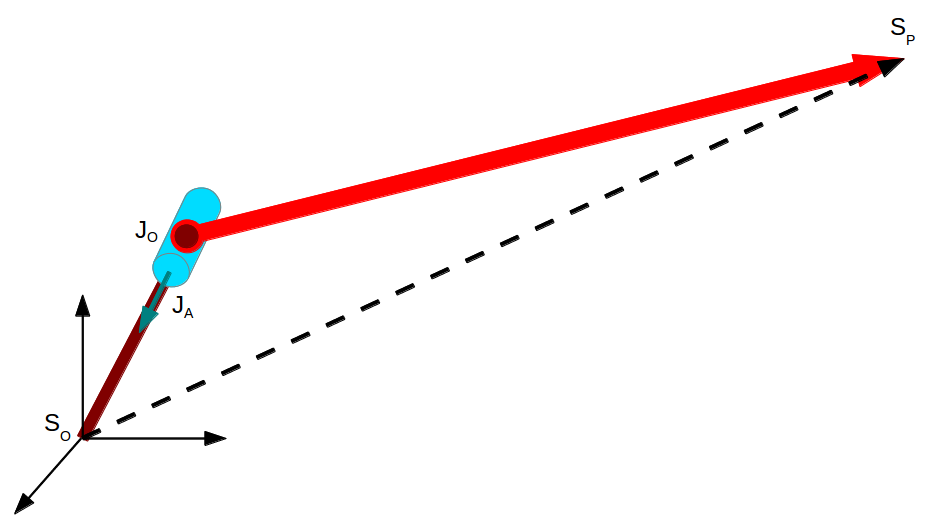
\includegraphics[width=0.75\textwidth]{Segment.png}
    \caption{Definition of a Segment in Kinematica}
   	\label{FIG_SEGMENT_DEFINITION}
\end{figure}

\noindent Each segment consists of a joint (brown) and a link (red). The joint itself may be offset (fixed) from the the Segment origin ($S_O$), with position $J_O$ (Joint Origin) and moves/rotates along/around a Joint Axis ($J_A$). The link is of a fixed length. The Segment Pose is defined as the pose of the tip of the segment ($S_P$) relative to the segment origin.

\begin{figure}[!htp]
	\centering
    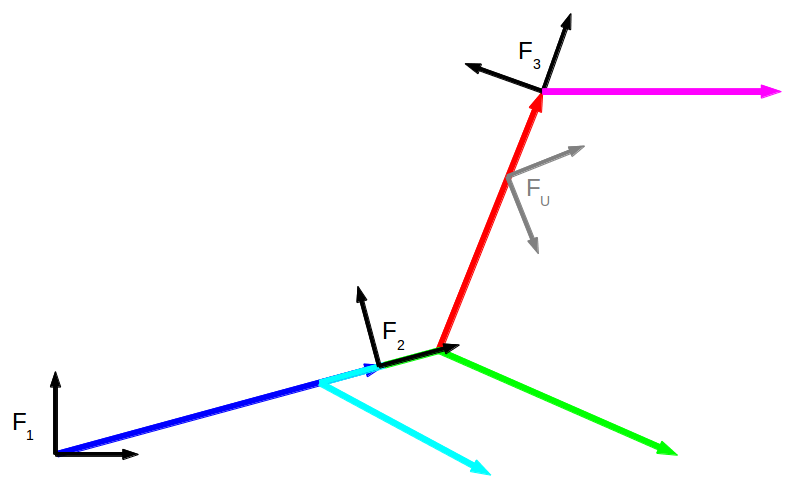
\includegraphics[width=0.75\textwidth]{Robot_Tree.png}
    \caption{Description of Robot in Kinematica}
   	\label{FIG_ROBOT_TREE_DEFINITION}
\end{figure}

\noindent A robot consists of a tree of such segments. In the original URDF, by definition, a tree is built by connecting segments to the \textbf{ends/tips} of parent segments as in Fig. \ref{FIG_ROBOT_TREE_DEFINITION}. In this case, the blue segment is taken as the root segment, with $F_1$ being the root frame of reference for the whole tree. Notice for example how all its children (cyan, green and red) are connected to its tip ($F_2$) although offset by some amount.

\subsection{Redefining the Root Frame}
When redefining the root frame, care must be taken regarding the direction of the segment links. Let us consider taking the red segment to be the new root link, with some frame on this segment $F_U$ as the root frame of reference. In this case, the blue segment will be connected to the base of the root, with its tip actually facing towards it rather than away from it. This is intentional and is retained to avoid confusion with redefining the tree structure/order. The rule to keep in mind is that whatever the root frame, the segments will:
\begin{enumerate}
\item Always have their origin frame at their base (this will be oriented with the tip of their \textbf{original} parent).
\item Always point in the same direction as defined by the original URDF file.
\item Always be defined by the pose of their tip, whether this is in a global or local frame of reference.
\end{enumerate}

\subsection{Computing Forward Kinematics}
There are two conventions when computing Forward Kinematics:
\begin{enumerate}
\item When requesting the `global' pose of a segment, this refers to the pose of the tip in the \textbf{user-defined root} frame of reference ($F_U$ in Fig \ref{FIG_ROBOT_TREE_DEFINITION}).
\item When requesting the pose of a segment with respect to some other segment (including the segment which `houses' the root), this refers to the pose of the tip of the first with respect to the \textbf{frame at the tip} of the second.
\end{enumerate}

\subsection{Computing Jacobians}
The next major component of the library is the computation of Jacobians. The library computes the First Order linear approximation to the Analytical Jacobian around a particular configuration. Consider Fig. \ref{FIG_EFF_JACOBIAN}. 

\begin{figure}[h]
\centering
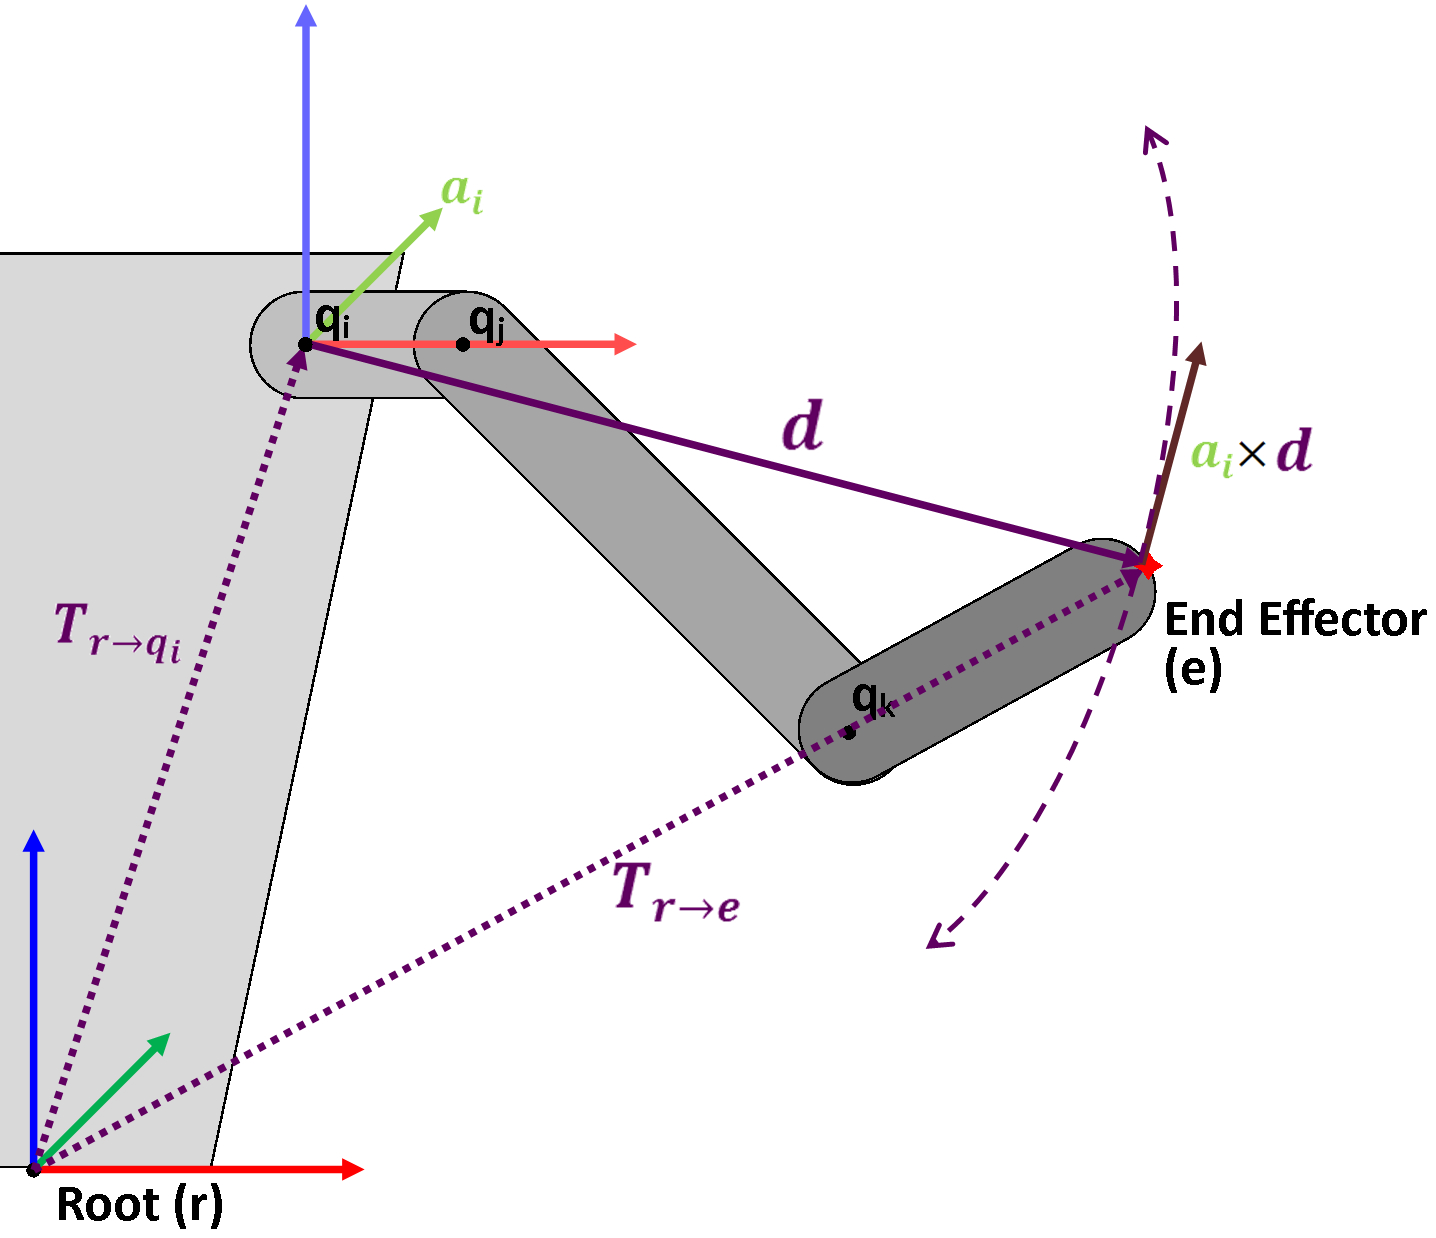
\includegraphics[width=0.7\textwidth]{EFF_Jacobian.png}
\caption{Derivation for the End-Effector Jacobian}
\label{FIG_EFF_JACOBIAN}
\end{figure}

\noindent Consider the computation of the Jacobian entry for End Effector (e) with respect to joint $q_j$ (column $J_e^{q_j}$), which is a revolving joint rotating about $a_j$ (specified in terms of the root frame). Fixing all other joints, different angles for $q_j$ will position $e$ on a circular path of radius $|d_j|$. In the neighbourhood of the current value for $q_j$, the change in position and hence the Jacobian entry for $q_j$ can be linearised to the cross product of $a_j$ and $d_j$ i.e.
\begin{equation}
J_e^{q_j} = a_j \times d_j \label{IK_CROSS}
\end{equation}
\begin{equation}
d = T_{r\rightarrow e} - T_{r\rightarrow q_i}
\end{equation} with $d$ being defined in the root frame.

\noindent The process is even simpler for prismatic joints. In this case, the joint axis (along which the joint slides) is directly the positional jacobian entry for that joint.

\newpage
\section{Using the Library}
This section describes general usage of the library, including installation, building, dependencies etc...

\subsection{Setup}
\subsubsection*{Pre-Requisites}
The Kinematica Library is designed to be as standalone a package as possible. Nevertheless, it does make use of a number of system dependencies:
\begin{itemize}
\item \textbf{Boost} Library for thread synchronisation
\item \textbf{Orocos KDL} which provides the base infrastracture.
\item \textbf{kdl\_parser}, a ROS package which is used to parse URDF files to construct the original KDL Tree.
\item \textbf{EIGEN} which is used for the matrix manipulations within the project
\end{itemize}
Moreover, although Kinematica is independent of ROS, it utilizes the ROS Catkin build system but this can be circumvented if needed by building using cmake. The only limitation is that it uses the \textbf{\textit{kdl\_parser}} package which is a ROS package: however, future implementations will attempt to address this.

\subsubsection*{Installation and Building}
The library is built from the source provided. Currently the Catkin build system is used, making for an easier integration with ROS packages. Alternatively if you wish to build it as a standalone system, you must modify the CMakeLists.txt file to accomodate the normal cmake conventions.

\subsubsection*{Notes}
The library tools exist within the \textbf{\textit{kinematica}} namespace. Usage of the library requires including the \textbf{\textit{``kinematica/KinematicTree.h''}} header file but that is all.\\
\\
\noindent Finally, the library is fully thread-safe in its current implementation.

\newpage
\subsection{Public API}
This section will guide the reader through general usage of the library.

\subsubsection*{Solution Parameters}
\label{SOLUTION_PARAMS}
The library consists of two main public data types. The first is a structure for setting solution parameters (in the interest of efficiency, we choose to pre-define these) and is described hereunder in Table \ref{TAB_SOLUTION_FORM_STRUCTURE}. The other is the actual KinematicTree class which is detailed in the next subsection.

\begin{table}[!htp]
\centerline
{
\begin{tabular}{|m{3.8cm}||m{2.1cm}|m{8cm}|}
\hline
\textbf{Parameter} & \textbf{Type} & \textbf{Description} \\
\hline
\hline
\textit{\textbf{root\_segment}} & std::string & The name of the segment to use as root. The empty string defaults to the URDF root. \\
\hline
\textit{\textbf{root\_seg\_off}} & KDL::Frame & The position of the root frame relative to the \textbf{tip} of \textit{root\_segment}.\\
\hline
\textit{\textbf{joints\_update}} & std::vector of std::string & Specifies which joints will be modified and in which order they will be specified. If the \textit{zero\_other\_joints} flag is not set, this vector must contain \textbf{all} the joints in the robot.\\
\hline
\textbf{\textit{zero\_other\_joints}} & bool & Indicates whether unspecified joints in the \textit{joints\_update} vector will be zeroed out in any kinematics computations. Any zeroed out joints will also not factor in the Jacobian computation.\\
\hline
\textbf{\textit{ignore\_unused\_segs}} & bool & Again an efficiency-related flag. If set, segments whose poses do not factor into any of the end-effectors specified for the Forward Kinematics/Jacobian computation (\textit{end\_effector\_segs}) are skipped in such calculations. Otherwise, all segments will be updated. \\
\hline
\textbf{\textit{end\_effector\_segs}} & std::vector of std::string & For batch computation of Forward Kinematics/Jacobians. Lists the set of segments to which the end-effectors are attached. Each segment may be used as many times as necessary (if for example, multiple end-effectors are connected to the same segment).\\
\hline
\textbf{\textit{end\_effector\_offs}} & std::vector of KDL::Frame & The pose of the end-effector w.r.t. the \textbf{tip} of the corresponding segment. The vector must be the same size as \textit{end\_effector\_segs} or left empty.\\
\hline
\end{tabular}
}
\caption{Definition of the \textbf{SolutionForm\_t} structure}
\label{TAB_SOLUTION_FORM_STRUCTURE}
\end{table}

\subsubsection*{The KinematicTree class}
The KinematicTree is designed to handle all low-level tasks involved in computing forward kinematics. Its usage will be introduced through the use of an example.\\
\newline
\noindent The first thing to do is to create the \textbf{\textit{SolutionForm\_t}} structure to specify the parameters we will be interested in. The reason for this is to provide more efficiency in cases where the same set of queries will be set (as in optimisation/control problems). Although these can be changed later on, constantly re-initialising with different parameters should be avoided: rather multiple objects should be instantiated. In this case we keep the same root as the URDF by passing in the empty string for \textit{root\_segment}. We also desire that the root is situated at the tip of the root segment (and hence we pass in the identity transformation).

\begin{lstlisting}
kinematica::SolutionForm_t solution_form;
  
solution_form.root_segment = ""; //!< Retain root joint
solution_form.root_seg_off = KDL::Frame::Identity();
\end{lstlisting}

\noindent We also must specify the joints we will be using: since we did not specify all joints, we set the flag to zero out unspecified joints\footnote{Note that the initialiser-list syntax requires C++11.}. 

\begin{lstlisting}
solution_form.joints_update = {"joint_1", "joint_3", "joint_4"}; //!< Fill joints
solution_form.zero_other_joints = true; //!< We have not specified all joints
\end{lstlisting}

\noindent Finally, we indicate the position of the end-effector we are interested in.

\begin{lstlisting}
solution_form.ignore_unused_segs = false; //!< Compute for all segments
solution_form.end_effector_segs.push_back("segment_4"); //!< End-effector
 
KDL::Frame eff_offs;          //!< Prepare frame for the end-effector offset
eff_offs.p = KDL::Vector(0.5, 0.1, 0.0);  //!< Translation component
eff_offs.M = KDL::Rotation::EulerZYZ(0.1, 0.2, 0.05); //!< Rotation component
solution_form.end_effector_offs.push_back(eff_offs);
\end{lstlisting}

\noindent Having prepared the initialisation parameters we may go ahead and create a KinematicTree object. We must pass two variables to the constructor: the \textbf{full} path to the urdf file, plus the initialisation structure we just defined.

\begin{lstlisting}
kinematica::KinematicTree robot_tree("robot.urdf", solution_form);
\end{lstlisting}
\noindent Alternatively, we may call the default constructor and initialise the class at a later stage by calling the \textbf{\textit{initKinematics(...)}} function, with the following signature:

\begin{lstlisting}
bool initKinematics(const std::string &, const SolutionForm_t &)
\end{lstlisting}
\noindent Again, the first parameter is the path of the urdf describing the robot, and the second the solution parameters. That is all as far as setup is concerned. Once the object has been initialised, Forward Kinematic computations may be invoked by calling:

\begin{lstlisting}
bool updateConfiguration(const Eigen::VectorXd &)
\end{lstlisting}
\noindent The function takes one argument, the Eigen::Vector of joint values. This vector must be the same size as the joints\_update vector defined previously and the joint values must be specified in the same order. This function will generate the internal computations to update the state of the tree structure based on the joint angles. Having done this, the user may request the actual \textbf{positions} of the pre-defined end-effectors by using:

\begin{lstlisting}
bool generateForwardMap()
\end{lstlisting}
\noindent If the function returns with success (true), the user may call
\begin{lstlisting}
bool getPhi(Eigen::VectorXd &)
\end{lstlisting}
to copy the result into the passed vector\footnote{Note that although the name refers to Forward Maps and $\Phi$, this is actually the result of the forward mapping and \textbf{not} the function itself: i.e. it gives the actual positions.}. The result will consist of the 3D \textbf{position} of each pre-defined end-effector, in the order specified in \textit{SolutionForm\_t::} \textit{end\_effector\_segs}. For convenience a wrapper function for the above two is also implemented which simultaneously generates and returns the forward-map vector:
\begin{lstlisting}
bool generateForwardMap(Eigen::VectorXd &)
\end{lstlisting}

\noindent Similarly the user may request computation of the position Jacobian\footnote{Currently, only the position Jacobian is implemented since in theory this can be used to implemented any other kinematic Jacobian by appropriate `trickery': in future implementations, this functionality may be extended.}, however, this will \textbf{only} be valid if the Forward Map was \textbf{previously generated}. Each column in the Jacobian represents the contribution of \textbf{only} those joints and specified in \textit{SimulationForm\_t::}\textit{joints\_update} with the same ordering. The rows on the other hand represent the effect on each position co-ordinate (3D) of each segment in the order specified by \textit{SolutionForm\_t::} \textit{end\_effector\_segs}. The functions are:

\begin{lstlisting}
bool generateJacobian()	// Generate Jacobian
bool generateJacobian(Eigen::MatrixXd &) // ... and pass result

bool getJacobian(Eigen::MatrixXd &)	// Get a pre-computed Jacobian
\end{lstlisting}

\noindent where again, the first two generate the Jacobian from the underlying kinematics and the last function simply gives a copy of the most recent Jacobian computation stored internally.\\
\\
\noindent We anticipate that in certain situations the state of the environment may change. To this end, a function is provided to update \textbf{only} the end-effector segments.
\begin{lstlisting}
bool updateEndEffectors(const SolutionForm_t &)
\end{lstlisting}
This function takes in a \textit{SolutionForm\_t} structure, but the only parameters which need to be set are:
\begin{itemize}
\item \textbf{ignore\_unused\_segs} flag
\item \textbf{end\_effector\_segs} vector (compulsary)
\item \textbf{end\_effector\_offs} vector (may be optionally left empty)
\end{itemize}
The elements have the same meaning as during initialisation.\\
\newline
\noindent In order to provide additional flexibility for the general user, arbitrary pose calculators are also implemented. Again, the \textbf{\textit{updateConfiguration(...)}} function must be called first. In this case, the \textit{ignore\_unused\_segs} flag must be \textit{false}, otherwise results might be invalid if the required pose is of a segment which itself does not affect the end-effectors specified. Four methods are provided, two taking string arguments and two taking integer index arguments: the latter two are much more efficient but the results are identical.\\

\begin{lstlisting}
bool getPose(std::string child, std::string parent, KDL::Frame& pose)
bool getPose(std::string child, KDL::Frame & pose)

bool getPose(int child, int parent, KDL::Frame & pose);
bool getPose(int child, KDL::Frame & pose);
\end{lstlisting}
\noindent In each case, the function requires the name/index of the query node (labelled \textit{child}) and optionally that of the node to use as reference frame (labelled \textit{parent}). If this is specified, the resulting frame is the pose of the \textbf{tip} of the child w.r.t. the \textbf{frame at the tip of the parent}. If the parent is omitted, the returned frame is the pose of the \textbf{tip} of the child w.r.t. the \textbf{root frame} (and \textbf{not} necessarily the tip of the root segment)\footnote{The major scenario where this is confusing is if the parent is the root segment itself. If the root segment name is specified the pose will be w.r.t. the tip of the root segment: if not, it will be w.r.t. the true root frame, which was specified in initialisation as an offset from the root segment tip.}. In each case the last argument is the place-holder for storing the result, since the return value is used to indicate success (true) or failure (false).\\
\newline
\noindent The mapping from segment names to segment indices may be obtained by calling (after appropriate initialisation) the function:

\begin{lstlisting}
bool getSegmentMap(std::map<std::string, int> &)
\end{lstlisting}

\noindent Finally, to support external traversal of the tree, the object offers functions to obtain the parent/children of a particular node. In each case, variants using string and integer input are provided, giving back names and indices respectively.

\begin{lstlisting}
std::string getParent(std::string child);
int         getParent(int         child);

std::vector<std::string> getChildren(std::string parent);
std::vector<int>         getChildren(int         parent);
\end{lstlisting}

\newpage
\section{The Kinematica Implementation}
This section contains more advanced concepts and is intended for future developpers/maintainers. As such, it describes the design decisions, computations etc... within the API.

\subsection{Major Design Decisions}
The purpose of Kinematica is to provide a generic but efficient Forward Kinematics library for robotic applications. This has led to certain design choices:
\begin{enumerate}
\item The library is targeted at optimisation problems, whereby in most cases, the computations center on the same subset of end-effectors. In light of this, we choose to specify such parameters during initialisation, since this is a performance-costly process. We also do some considerable pre-processing during this stage.
\item We favour memory use over re-computations wherever applicable, on the assumption that matrix operations are resource intensive and that several end-effectors might require the same subset of data within one iteration.
\item Almost all functions indicate success or failure through a boolean return value (True/False respectively).
\item Efficiency comes second only to thread-safety and proper information hiding, so that the library can be used by non-expert software engineers. The rule is that:
\begin{itemize}
\item Public Methods (accept for constructor) are THREAD-SAFE through a \textbf{common} mutex.
\item Private Methods are inherently NOT THREAD-SAFE.
\end{itemize}The motivation is that public functions may internally make use of multiple private functions (so locking would block). However, since the public methods do not spawn any threads, thread-safety is maintained.
\end{enumerate}
The overall architecture consists of the \textbf{KinematiceTree} class which encapsulates all the functionality plus a number of structures for data organisation and some helper functions.

\subsection{Data Types and Auxiliaries}

\subsubsection*{Structures}
There are three main data types apart from the Kinematics Class itself.\\
\newline
The \textbf{SolutionForm\_t} structure was defined within the \textbf{Using the Library} section. Refer to subsection \ref{SOLUTION_PARAMS}.\\
\newline
The \textbf{KinematicElement\_t} structure is used to define our notion of a tree element. Due to the potential change of root, it was decided to build our own tree structure. Table \ref{TAB_KINEMATIC_ELEMENT_STRUCTURE} describes each element.\\
\newline
Finally, the \textbf{JointType\_t} enum, defines the three types of joints supported by Kinematica:
\begin{itemize}
\item \textbf{\textit{JNT\_UNUSED}} : An unused/undefined joint.... typically this is a fixed joint.
\item \textbf{\textit{JNT\_PRISMATIC}} : A prismatic joint (sliding)
\item \textbf{\textit{JNT\_ROTARY}} : A rotary joint
\end{itemize}

\begin{table}[!htp]
\caption{Definition of the \textbf{KinematicElement\_t} structure}
\centerline
{
\begin{tabular}{|m{2.5cm}||m{3.0cm}|m{8cm}|}
\hline
\textbf{Parameter} & \textbf{Type} & \textbf{Description} \\
\hline
\hline
\textit{\textbf{segment}} & KDL::Segment & Our copy of the KDL::Segment, used to compute local (within segment) forward kinematics computation based on joint values. \\
\hline
\textit{\textbf{needed}} & bool & Efficiency flag: indicates whether the contribution of this segment is necessary for the queries the library will be set. \\
\hline
\textit{\textbf{parent}} & int & Index into the vector of Kinematic Elements pointing to the parent (of the new tree structure) of this node. For the Root node, will have the value -1. \\
\hline
\textit{\textbf{from\_tip}} & bool & Flag for indicating the traversal of segments (due to change of roots). True signifies that we are connected to \textit{parent} from its tip (as is normal): otherwise we are connected to its base.\\
\hline
\textit{\textbf{to\_tip}} & bool & Flag for indicating the traversal of segments: True indicates that we are moving towards the tip of the segment and False v.v. \\
\hline
\textit{\textbf{joint\_type}} & kinematica:: JointType\_t & Defines the type of joint we are dealing with (refer to the enum definition for more information).\\
\hline
\textit{\textbf{joint\_index}} & int & Index for this segment's joint into the configuration array specified by the user. Note that this (and all joint-related members) refer to the \textbf{original} joint associated with this \textit{segment}.\\
\hline
\textit{\textbf{tip\_pose}} & KDL::Frame & The latest update of the pose of the \textbf{tip} of this segment w.r.t. the \textbf{root frame}.\\
\hline
\textit{\textbf{joint\_pose}} & KDL::Frame & This is the pose of the \textbf{base} of the segment as a whole ($S_O$ in Fig. \ref{FIG_SEGMENT_DEFINITION}) with respect to the \textbf{root frame}.\\
\hline
\textit{\textbf{joint\_origin}} & Eigen::Vector3d & The latest update of the \textbf{position} of the joint's origin ($J_O$ in Fig. \ref{FIG_SEGMENT_DEFINITION}) in the \textbf{root frame}.\\
\hline
\textit{\textbf{joint\_axis}} & Eigen::Vector3d & The Joint Axis of rotation (Fig. \ref{FIG_SEGMENT_DEFINITION}, $J_A$), oriented w.r.t. the root frame.\\
\hline
\textit{\textbf{child}} & std::vector of int & Indices (within the vector of Kinematic Elements) of (any) children of this node: these are the children in the \textbf{new} tree structure.\\
\hline
\end{tabular}
}
\label{TAB_KINEMATIC_ELEMENT_STRUCTURE}
\end{table}

\subsubsection*{Helper Functions}

\textcolor{blue}{Eigen::Vector3d} \textbf{vectorKdlToEigen}(\textcolor{DarkGreen}{const} \textcolor{blue}{KDL::Vector \&} kdl\_vec)\\
\noindent This Function converts between the two main position types in the library, namely from \textit{KDL::Vector} to \textit{Eigen::Vector3d}.\\
\newline
\begin{lstlisting}
bool recursivePrint(kinematica::KinematicTree & robot, std::string node, std::string tab)
\end{lstlisting}
This is a debugging function and recursively prints the tree structure of a KinematicTree object, passes by reference as the first parameter, the current node (by name: start at the root), and the current preceding tab-width. The last parameter is used to provide a more intuitive display in characters, and in the first call to the function should be an empty string.\\
\newline
\noindent The logic behind the \textit{tab} field is as follows:
\begin{itemize}
\item If it is the empty string, then this is the root and the node name is printed.
\item Otherwise, print the `elbowed' arrow, taking care to avoid printing the vertical line multiple times.
\end{itemize}
Now depending on the number of children:
\begin{itemize}
\item If no children, this is the base case and we return.
\item If not, then increase indent and:
\begin{itemize}
\item If only one child, we append just a space (so that the recursive call will do the full elbow)
\item If more children, then we need to append a vertical line so that the remaining children will still be connected.
\end{itemize}
\end{itemize}
Finally, we recurse on all the children, removing the vertical line from the last one (since there will be no trailing siblings under it).

\subsection{Class Attributes}
All the class attributes are declared private to enforce information hiding and thread-safety: where necessary, access to the underlying variables is through getter/setter functions. These are displayed in table \ref{TAB_KINEMATIC_TREE_ATTRIBUTES}.

\begin{table}[!htp]
\caption{The Attributes of \textbf{KinematicTree}: KE\_t signifies KinematicElement\_t}
\centerline
{
\begin{tabular}{|m{3.25cm}||m{3.5cm}|m{7cm}|}
\hline
\textbf{Parameter} & \textbf{Type} & \textbf{Description} \\
\hline
\hline
\textit{\textbf{robot\_tree\_}} & std::vector $<$KE\_t$>$ & Holds the segments making up the tree structure. Numeric indexing provides an efficient implementation (over maps).\\
\hline
\textit{\textbf{segment\_map\_}} & std::map $<$std::string, int$>$ & Maps from segment names to indices into \textit{robot\_tree\_} for convenience.\\
\hline
\textit{\textbf{zero\_undef\_jnts\_}} & bool & Flag with same meaning as \textit{SolutionForm\_t::zero\_other\_joints}.\\
\hline
\textit{\textbf{num\_jnts\_spec\_}} & int & (For Error-checking) The size of the expected configuration (joint-values) vector.\\
\hline
\textit{\textbf{eff\_segments\_}} & std::vector $<$int$>$ & The list of end-effector segments (same as \textit{SolutionForm\_t::end\_effector\_segs} but transformed into numeric indices).\\
\hline
\textit{\textbf{eff\_seg\_offs\_}} & std::vector $<$KDL::Frame$>$ & The set of end-effector offsets (may be empty: same as \textit{SolutionForm\_t::end\_effector\_offs}).\\
\hline
\textit{\textbf{forward\_map\_}} & Eigen::VectorXd & Internal copy of the most recent $\Phi$ vector containing the poses of the end effectors.\\
\hline
\textit{\textbf{jacobian\_}} & Eigen::MatrixXd & Internal copy of the most recent Jacobian computation.\\
\hline
\textit{\textbf{member\_lock\_}} & boost::mutex & Lockable mutex for thread-safety and synchronisation.\\
\hline
\end{tabular}
}
\label{TAB_KINEMATIC_TREE_ATTRIBUTES}
\end{table}



\subsection{Initialisers}
This subsection introduces the initialisation-related functions.

\subsubsection*{Constructors}
A default and two initialisation constructors are provided.
\begin{lstlisting}
KinematicTree(void);
KinematicTree(const std::string & , const SolutionForm_t & );
KinematicTree(const KDL::Tree & , const SolutionForm_t & );
\end{lstlisting}
The initialisation constructors take two parameters.
\begin{enumerate}
\item The path to the URDF-file containing the robot description in the first case and the pre-initialised KDL::Tree in the second.
\item The structure of solution parameters.
\end{enumerate}
which it then passes to the \textbf{\textit{initKinematics(...)}} function. All constructors are guaranteed to initialise the object in a stable state\footnote{By this we mean that the object has all its members initialised to default values such as empty vectors, reset flags etc.}.

\subsubsection*{initKinematics}
These functions provide a thread-safe wrapper for a private common initialise function (to allow flexibility in initialising from a urdf file or a KDL::Tree). Their signature is similar to the initialisation constructors (above), with success or failure being indicated through the return value (True/False respectively).
\begin{lstlisting}
bool initKinematics(const std::string &, const SolutionForm_t &);
bool initKinematics(const KDL::Tree &, const SolutionForm_t &);
\end{lstlisting}

\subsubsection*{initialise}
This is the private common wrapper for initialising the object from a KDL::Tree, and the Solution Form parameters. 
\begin{lstlisting}
bool initKinematics(const KDL::Tree &, const SolutionForm_t &);
\end{lstlisting}
In order, the function:
\begin{enumerate}
\item Cleans up the internal data members.
\item Calls \textbf{\textit{buildTree(...)}} to build the internal tree structure, potentially changing the root.
\item Sets the joint ordering that will be used using \textit{\textbf{setJointOrder(...)}}.
\item Calls \textbf{\textit{setEndEffectors(...)}} to settle end-effector constants/indices.
\end{enumerate}
If any of the sub-methods fail, all data members are cleaned up and the function returns. Success or failure is indicated.

\subsubsection*{buildTree}
This is a private (non-thread-safe) function, which aims to build the tree structure using the user-defined segment/frame as root.
\begin{lstlisting}
bool buildTree(const KDL::Tree &, std::string, std::map<std::string, int> &);
\end{lstlisting}
The three arguments are:
\begin{enumerate}
\item The KDL::Tree structure previously loaded
\item The name of the segment to use as root
\item Placeholder for building the joint map (from joint name to the index into the \textit{robot\_tree\_} vector corresponding to the segment to which the joint pertains)
\end{enumerate}
In order to ensure that the passed segment does indeed exist, we take a detour by first requesting the whole map of segments from the KDL::Tree and then attempting to \textit{find()} the segment (rather then just dereferencing it). The tree is then built in a recursive manner through the \textbf{\textit{addSegment(...)}} function (see below).

\subsubsection*{addSegment}
This is a recursive private (non-thread-safe) function which traverses the \textbf{original} tree and converts it into the new-rooted structure.\\
\newline
\noindent Consider the simplified robot description, replicated hereunder as Fig. \ref{FIG_ROBOT_TREE_DEFINITION_2}. Assume that initially the root segment is the blue one, with $F_1$ being the associated root frame (the base of the segment), and that we now wish the red segment to be our new root, with the actual frame at $F_U$. In starting from the (new) root node, we  need to consider three cases:
\begin{itemize}
\item The \textbf{Root} segment: then all segments attached to it will become its children: this includes its original children, its original parent as well as its original siblings (children of the same parent). In this example, this amounts to all the segments!
\item We are moving \textbf{along the original tree direction} (such as for the magenta segment): then the structure remains the same (parents remain parents, children remain children).
\item We are moving \textbf{against the original tree direction}: in this case both the original parent and the siblings become children in the new tree. For example, moving from red to blue, the parent (originally blue) becomes a child, as do the cyan and green segments since these are siblings.
\end{itemize}

\begin{figure}[!htp]
	\centering
    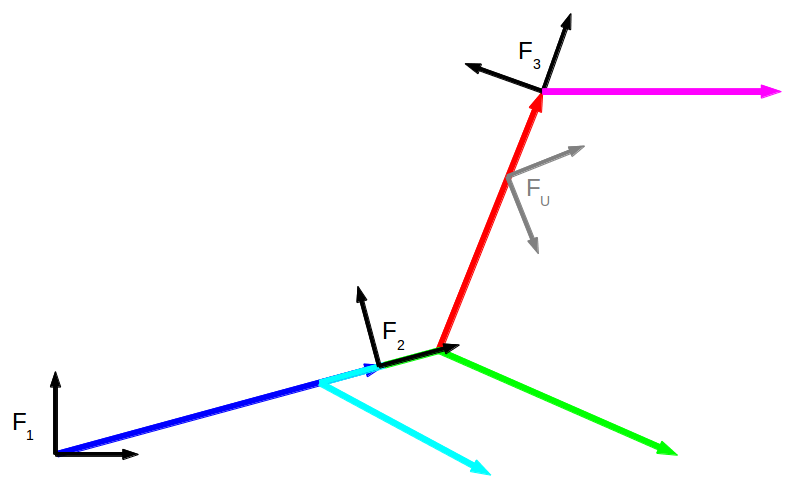
\includegraphics[width=0.75\textwidth]{Robot_Tree.png}
    \caption{Description of Robot in Kinematica}
   	\label{FIG_ROBOT_TREE_DEFINITION_2}
\end{figure}

\noindent The function has the following signature:
\begin{lstlisting}
bool addSegment(KDL::SegmentMap::const_iterator, int, int &, bool, bool, const std::string &, std::map<std::string, int> &)
\end{lstlisting}
with the following parameters:
\begin{enumerate}
\item Iterator to the next element in the \textbf{original} KDL::Tree
\item Index into the new \textit{robot\_tree\_} pointing to the parent to which this segment will be child.
\item Placeholder for the position of this segment (once it is created) within the \textit{robot\_tree\_} (since the parent will need references to its children).
\item Indicator whether this segment is connected to its \textbf{new} parent through the parent's tip (True) or base (False).
\item Indicator whether we are moving towards the tip of this segment (True) or towards its base (False).
\item Name of the original root (for checking)
\item Reference to the joint map (for updating)
\end{enumerate}
The function first creates a new Kinematic Element with default values and pushes it into the \textit{robot\_tree\_} vector. This ensures that:
\begin{itemize}
\item The new root segment is \textbf{always} at index 0 (for consistency).
\item The segment ordering is such that a child \textbf{never} appears before its (new) parent. This is necessary for the efficient and correct updating of Forward Kinematics.
\end{itemize}
It also records the index in the \textit{segment\_map\_} and updates the \textit{joint\_map} to associate the joint name with its original segment. The three scenarios are identified through the use of the direction flags (with the root using a special invalid combination `true/false'). The function then iterates through the \textbf{original} children of this segment (and optionally the parent) and calls itself recursively on each. Finally, it assigns the returned child index to the respective segment (due to conditions 1 and 3). Checks are carried out to ensure that we do not dereference the parent of the original root (which does not exist).

\subsubsection*{setJointOrder}
This function iterates through all the segments in \textit{robot\_tree\_}, specifying whether this joint will be controlled or not (through the \textit{joint\_type} paramater) and if it will be controlled, what type it is and the index into the array the user will use to specify the joint values. This is built using the previously generated \textit{joint\_map} and the vector of joint names in \textit{SolutionForm\_t::joints\_update}. The signature is:
\begin{lstlisting}
bool setJointOrder(const std::vector<std::string> &, bool, const std::map<std::string, int> &);
\end{lstlisting}
with the parameters:
\begin{itemize}
\item Vector of joint names in the order they will be specified
\item Flag to indicate whether unspecified joints should be zeroed out: if not set and not all the joints are specified the function fails.
\item The joint map previously generated.
\end{itemize}

\subsubsection*{setEndEffectors}
This is the last function to be called during initialisation: it is a private non-thread-safe function taking the \textit{SolutionForm\_t} specification as parameter, and returning an indication of success/failure.
\begin{lstlisting}
bool setEndEffectors(const SolutionForm_t &);
\end{lstlisting}
It initialises the root segment's tip pose (since this will be constant) and then populates the vector of segment indices which will be used for computation of end-effector forward kinematics and jacobians. It makes use of the \textit{\textbf{recurseNeedFlag()}} function to specify that this segment and all its parents up to the root are required for computation. It also pre-allocates memory for the forward map and jacobian matrices.

\subsubsection*{recurseNeedFlag}
As the name implies this is a recursive function, with the aim of traversing up the tree from a segment all the way to the root, setting the \textit{needed} flag for the corresponding segment. It takes in one parameter (the index of the segment in the \textit{robot\_tree\_} vector) and calls itself recursively until the root is reached.
\begin{lstlisting}
bool recurseNeedFlag(int);
\end{lstlisting}

\subsubsection*{isInitialised}
Coming Soon

\subsection{Updaters}
The following set of functions are expected to be called repeatedly during iterations to update the state of the kinematic tree.

\subsubsection*{updateConfiguration}
Coming Soon

\subsubsection*{generateForwardMap}
Coming Soon

\subsubsection*{computePhi}
Coming Soon

\subsubsection*{generateJacobian}
Coming Soon

\subsubsection*{computeJacobian}
Coming Soon

\subsection{Accessors}
These functions provide access to the underlying data structures. Usually, they must be called after appropriate initialisation/updating for the results to be correct.

\subsubsection*{getJacobian}
Coming Soon

\subsubsection*{getPhi}
Coming Soon

\subsubsection*{getPose}
Coming Soon

\subsubsection*{getSegmentMap}
Coming Soon

\subsubsection*{getParent}
Coming Soon

\subsubsection*{getChildren}
Coming Soon


\newpage
\appendix
\section{Known Limitations}
\begin{enumerate}
\item There is currently no collision-detection support
\end{enumerate}

\section{Version History}

\begin{table}[!htp]
\centerline
{
	\begin{tabular}{|m{2.0cm}||m{6cm}|m{6cm}|}
	\hline
	\textbf{Version} & \textbf{Library Changes} &  \textbf{Documentation Changes}\\
	\hline
	\hline
	\center{\textbf{0.0.1}} & \begin{itemize}[leftmargin=0.35cm]
					\item First Iteration of Kinematica
					\end{itemize}
				  & \begin{itemize}[leftmargin=0.35cm]
				    \item First Documentation
				  	\end{itemize}\\
	\hline	
	\center{\textbf{1.0.0 (Marvin)}} & \begin{itemize}[leftmargin=0.35cm]
					\item First Official Release
					\item Deprecated the \textbf{\textit{KinematicsType\_t}} enum
					\item Added Support for initialisation directly from KDL::Tree object.
					\item Extensively Tested and Debugged
					\end{itemize}
				  & \begin{itemize}[leftmargin=0.35cm]
				    \item Clarified some concepts in the Public API
				    \item Documenting Detailed API for developers (in progress)
				  	\end{itemize}\\
	\hline	
	\center{\textbf{1.1.0}} & \begin{itemize}[leftmargin=0.35cm]
					\item Added support for prismatic joints: fixed joints should be simply ignored by the user
					\end{itemize}
				  & \begin{itemize}[leftmargin=0.35cm]
				    \item Clarified the changes in the documentation
				  	\end{itemize}\\
	\hline
	\center{\textbf{1.2.0}} & \begin{itemize}[leftmargin=0.35cm]
					\item Added ability to change the configuration of end-effectors as needed.
					\end{itemize}
				  & \\
	\hline
	\end{tabular}
}
\end{table}

\end{document}